
%(BEGIN_QUESTION)
% Copyright 2006, Tony R. Kuphaldt, released under the Creative Commons Attribution License (v 1.0)
% This means you may do almost anything with this work of mine, so long as you give me proper credit

Beregn verdiene i kalibreringstabellen under for en transmitter som måler væskegrensesnitt (spesifikke vekter = 0.75 og 1.2), med kalibreringstoleranse $\pm$ 0.1\%.  Angi hvilken port på $\Delta$P-transmitteren kalibreringstrykket skal påføres:

$$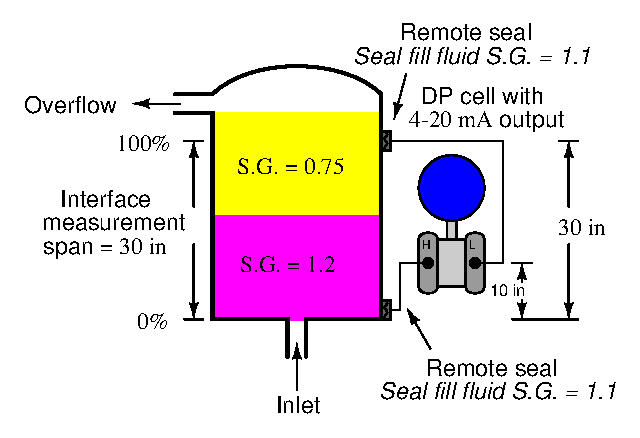
\includegraphics[width=15.5cm]{i00311x01.eps}$$

% No blank lines allowed between lines of an \halign structure!
% I use comments (%) instead, so that TeX doesn't choke.

$$\vbox{\offinterlineskip
\halign{\strut
\vrule \quad\hfil # \ \hfil & 
\vrule \quad\hfil # \ \hfil & 
\vrule \quad\hfil # \ \hfil & 
\vrule \quad\hfil # \ \hfil & 
\vrule \quad\hfil # \ \hfil & 
\vrule \quad\hfil # \ \hfil \vrule \cr
\noalign{\hrule}
%
% First row
Grensesnitt- & Prosent av & $\Delta$ trykk & Utgangssignal & Utgangssignal & Utgangssignal \cr
%
% Another row
nivå (in) & spenn (\%) & målt ("W.C) & ideelt (mA) & min. (mA) & maks. (mA) \cr
%
\noalign{\hrule}
%
% Another row
  & 0 &  &  &  &  \cr
%
\noalign{\hrule}
%
% Another row
  & 10 &  &  &  &  \cr
%
\noalign{\hrule}
%
% Another row
  & 25 &  &  &  &  \cr
%
\noalign{\hrule}
%
% Another row
  & 50 &  &  &  &  \cr
%
\noalign{\hrule}
%
% Another row
  & 75 &  &  &  &  \cr
%
\noalign{\hrule}
%
% Another row
  & 90 &  &  &  &  \cr
%
\noalign{\hrule}
%
% Another row
  & 100 &  &  &  &  \cr
%
\noalign{\hrule}
} % End of \halign 
}$$ % End of \vbox

\vskip 10pt

Vis all matematisk utregning slik at instruktøren kan kontrollere den konseptuelle gyldigheten av metoden(e) dine.  En god kontroll er å verifisere at alle mellomregninger har fysisk mening.  {\bf Hvis du virkelig forstår hva du gjør, vil du kunne identifisere riktig måleenhet for hvert mellomresultat og vise hvor tallet gjelder i scenariet}.

\vskip 20pt \vbox{\hrule \hbox{\strut \vrule{} {\bf Forslag til sokratisk diskusjon} \vrule} \hrule}

\begin{itemize}
\item{} Spiller transmitterens plassering innenfor 30-tommersområdet noen rolle?  Ville kalibreringen endres om transmitteren flyttes 5 tommer opp, uten å flytte fjernforseglingene?  Hvorfor/hvorfor ikke?
\item{} Anta at prosesskaret ikke fylles helt opp til overløpet.  Hvordan påvirker dette nøyaktigheten?  Vil transmitteren vise falskt lavt, falskt høyt, eller fortsatt riktig?
\item{} Demonstrer hvordan man kan {\it estimere} numeriske svar uten kalkulator.
\end{itemize}

\underbar{file i00311}
%(END_QUESTION)





%(BEGIN_ANSWER)

{\bf Delvis svar:}

% No blank lines allowed between lines of an \halign structure!
% I use comments (%) instead, so that TeX doesn't choke.

$$\vbox{\offinterlineskip
\halign{\strut
\vrule \quad\hfil # \ \hfil & 
\vrule \quad\hfil # \ \hfil & 
\vrule \quad\hfil # \ \hfil & 
\vrule \quad\hfil # \ \hfil & 
\vrule \quad\hfil # \ \hfil & 
\vrule \quad\hfil # \ \hfil \vrule \cr
\noalign{\hrule}
%
% First row
Grensesnitt- & Prosent av & $\Delta$ trykk & Utgangssignal & Utgangssignal & Utgangssignal \cr
%
% Another row
nivå (in) & spenn (\%) & målt ("W.C) & ideelt (mA) & min. (mA) & maks. (mA) \cr
%
\noalign{\hrule}
%
% Another row
 & 0 & 10.5 L &  &  &  \cr
%
\noalign{\hrule}
%
% Another row
 & 10 &  & 5.6 &  &  \cr
%
\noalign{\hrule}
%
% Another row
7.5 & 25 &  &  &  &  \cr
%
\noalign{\hrule}
%
% Another row
 &  & 3.75 L &  &  &  \cr
%
\noalign{\hrule}
%
% Another row
 & 75 &  &  & 15.984 &  \cr
%
\noalign{\hrule}
%
% Another row
 & 90 & &  &  & 18.416 \cr
%
\noalign{\hrule}
%
% Another row
30 & 100 &  & &  &  \cr
%
\noalign{\hrule}
} % End of \halign 
}$$ % End of \vbox

Merk: bokstaven ``L'' etter differansetrykkverdien betyr at dette positive trykket påføres transmitterens {\it low}-port.

%(END_ANSWER)





%(BEGIN_NOTES)

\noindent
{\bf LRV-betingelse:}

Det er 30 tommer lett væske (SG = 0.75) på transmitterens ``H''-port og 30 tommer fyllvæske (SG = 1.1) på ``L''-porten.  Differansetrykket ved LRV blir derfor:

$$\hbox{DP}_{LRV} = \left(30 \hbox{ in} \over 1 \right) \left(0.75 \hbox{ in water} \over 1 \hbox{ in liquid} \right) - \left(30 \hbox{ in} \over 1 \right) \left(1.1 \hbox{ in water} \over 1 \hbox{ in liquid} \right) $$

$$\hbox{DP}_{LRV} = (22.5 \hbox{ "WC}) - (33 \hbox{ "WC}) = -10.5 \hbox{ "WC}$$

\vskip 10pt

\noindent
{\bf URV-betingelse:}

Det er 30 tommer tung væske (SG = 1.2) på ``H''-porten og 30 tommer fyllvæske (SG = 1.1) på ``L''-porten.  Differansetrykket ved URV blir derfor:

$$\hbox{DP}_{LRV} = \left(30 \hbox{ in} \over 1 \right) \left(1.2 \hbox{ in water} \over 1 \hbox{ in liquid} \right) - \left(30 \hbox{ in} \over 1 \right) \left(1.1 \hbox{ in water} \over 1 \hbox{ in liquid} \right) $$

$$\hbox{DP}_{URV} = (36 \hbox{ "WC}) - (33 \hbox{ "WC}) = +3.0 \hbox{ "WC}$$

De to kapillarrørene til fjernforseglingene gir samlet et konstant trykk på $-33$ "WC til DP-transmitteren, uavhengig av transmitterens høyde relativt til prosesstanken.  Hvis transmitteren heves, reduseres fyllvæskens hydrostatiske trykk på ``L''-siden, men dette matches nøyaktig av tilsvarende økt sugetrykk (negativt trykk) på ``H''-siden.

Det bør også bemerkes at all prosessvæske over øvre fjernforsegling er irrelevant, fordi dette hydrostatiske trykket påvirker både ``H'' og ``L'' likt og derfor kanselleres (dvs. trykket over øvre fjernforsegling er {\it common-mode} og registreres ikke av DP-transmitteren).

% No blank lines allowed between lines of an \halign structure!
% I use comments (%) instead, so that TeX doesn't choke.

$$\vbox{\offinterlineskip
\halign{\strut
\vrule \quad\hfil # \ \hfil & 
\vrule \quad\hfil # \ \hfil & 
\vrule \quad\hfil # \ \hfil & 
\vrule \quad\hfil # \ \hfil & 
\vrule \quad\hfil # \ \hfil & 
\vrule \quad\hfil # \ \hfil \vrule \cr
\noalign{\hrule}
%
% First row
Grensesnitt- & Prosent av & $\Delta$ trykk & Utgangssignal & Utgangssignal & Utgangssignal \cr
%
% Another row
nivå (in) & spenn (\%) & målt ("W.C) & ideelt (mA) & min. (mA) & maks. (mA) \cr
%
\noalign{\hrule}
%
% Another row
0 & 0 & 10.5 L & 4 & 3.984 & 4.016 \cr
%
\noalign{\hrule}
%
% Another row
3 & 10 & 9.15 L & 5.6 & 5.584 & 5.616 \cr
%
\noalign{\hrule}
%
% Another row
7.5 & 25 & 7.125 L & 8 & 7.984 & 8.016 \cr
%
\noalign{\hrule}
%
% Another row
15 & 50 & 3.75 L & 12 & 11.984 & 12.016 \cr
%
\noalign{\hrule}
%
% Another row
22.5 & 75 & 0.375 L & 16 & 15.984 & 16.016 \cr
%
\noalign{\hrule}
%
% Another row
27 & 90 & 1.65 H & 18.4 & 18.384 & 18.416 \cr
%
\noalign{\hrule}
%
% Another row
30 & 100 & 3.0 H & 20 & 19.984 & 20.016 \cr
%
\noalign{\hrule}
} % End of \halign 
}$$ % End of \vbox

%INDEX% Measurement, interface level: calibration table

%(END_NOTES)
